\documentclass[12pt]{article}
\usepackage[reqno]{amsmath}
\usepackage{amsfonts}
\usepackage{mathtools}
\usepackage{amssymb}
\usepackage{amsthm}
%\usepackage{multicol}
\usepackage[a4paper, margin=1in]{geometry}
\usepackage{indentfirst}
\usepackage{bm}
\usepackage{hyperref}
\hypersetup{
    colorlinks=true,
    linkcolor=blue,      
    urlcolor=cyan,
}
\renewcommand{\thesection}{\Roman{section}}
\setlength{\parindent}{4em}


\begin{document}

\begin{center}
\par\noindent\rule{\textwidth}{0.6pt}\\[0.3cm]
\textbf{\LARGE{Assignment 1}}\\[0.3cm]
\Large{BT1010 : Introduction to Life Sciences}\\[0.1cm]
\large{April 5, 2021}\\[0cm]
\par\noindent\rule{\textwidth}{0.6pt}
\end{center}
%\begin{multicols}{2}
\noindent
\hspace{0.4cm}Name : Taha Adeel Mohammed
\par \noindent
\hspace{0.4cm}Roll No. : CS20BTECH11052
\section*{Superb Swimmers}
\noindent\fbox{%
    \parbox{\textwidth}{\; \\[-1mm]
    \large{
        Explain the fluid dynamic of \textbf{metachronal wave} to generate thrust?}\\[-4mm]
    }%
}
\par \vspace{4mm}
%Many diverse marine animals have converged upon a common swimming strategy using multiple propulsors, e.g. limbs or ctenes(rows of cilia), which move with metachronal waves to generate thrust. A single beat cycle consists of an effective stroke\ power stroke in which the extended cilium makes an oar-like movement towards one side, and a recovery stroke in which the cilium moves back by propagating a bend from base to tip(\ref{}). The rows of propulsors do this in a sequential manner(out of phase w.r.t their neighbours), rather than synchronously, giving rise to metachronal waves.  A metachronal wave is called symplectic(front to back) when it propagates in the direction of the effective stroke and it is called antiplectic(back to front) when the wave propagates in the direction opposite to the effective stroke. Back-to-front (antipletic) swimming pattern is thought to be more efficient than front-to-back or synchronous pattern, as we shall see.
At the single propulsor level, it has been observed that the  limbs/cilia of different marine animals using metachronal waves bent similarly during their power stroke\footnote{ A single beat cycle consists of an effective stroke/power stroke in which the extended propulsor makes an oar-like movement towards one side, and a recovery stroke in which the propulsor moves back by propagating a bend from base to tip}, that is, inflexion point occurs \texttt{$\sim$} $ 0.65$ along propulsor, and they bent $\sim 27^{\circ}$.  This helps encourages vortex formation on the leeward side of the propulsor(See Fig 2). Counter-rotating vortexes formed on the leeward side of a bending propulsor accelerate fluid at the intersection of the vortexes, and hence the  water flow is greater on the leeward side of the limb/cilia than the flowward side. So by Bernoulli's Principle, pressure at the leeward side is lesser(\textbf{negative pressure}), and this pressure gradient ultimately gives the thrust. So unlike conventionally thought that these pressure fields are dominated by positive pressure generated as a propulsor pushes on the water and pushes the swimmer forward, it is actually negative pressure fields aligned along the leeward side of moving propulsors that dominates the pressure field and serve to essentially pull animals through the water (termed \textbf{suction thrust}). Relying on negative pressure, as opposed to high pushing pressure enables these swimmers to exploit readily produced hydrodynamic structures and facilitates metachronal waves.\\
\par In addition to the benefits for single propulsors, negative pressure fields facilitate the movement and coordination of multiple propulsors which have antiplectic\footnote{A metachronal wave is called symplectic(front to back) when it propagates in the direction of the effective stroke and it is called antiplectic(back to front) when the wave propagates in the direction opposite to the effective stroke. Back-to-front (antipletic) swimming pattern is more efficient and widespread than front-to-back or synchronous pattern} metachronal wave kinematics. During an antiplectic metachronal wave, a leading propulsor will begin the power stroke and, after it has initiated its stroke, the propulsor immediately behind it will initiate its own power stroke. This sequential pattern will continue for all the subsequent propulsors in the antiplectic wave. Antiplectic metachronal waves enable each propulsor to \textbf{move unobstructed} by adjacent propulsors. The predominately negative pressure on the leeward of each propulsor serves to facilitate the kinematics of the adjacent propulsor by \textbf{reducing the hydrodynamic resistance} necessary to initiate and complete its power stroke. In addition, the negative pressure in the gap between adjacent propulsors can \textbf{serve as a cue} for the adjacent propulsor to initiate its power stroke. Hence this way of propulsion leads to enhanced thrust and hydrodynamic efficiency.\\
\begin{figure}[h!]
    \centering
      \frame{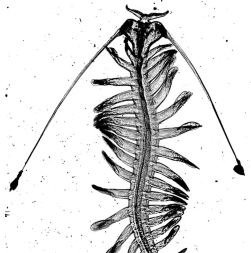
\includegraphics[width=\textwidth /3]{Figures/Annelid.png}}
      \caption{\textbf{Annelid} - \textit{Tomopteris sp.}}
      \label{Annelid}
\end{figure}
\par Taking the example of the polychaete annelid \textit{Tomopteris sp.}(See Fig \ref{Annelid}), and its vorticity\footnote{A vector that gives the  measure of local rotation of the fluid.}, pressure, and force graphs during the metachronal waves, we can better visualize and understand the above two paragraphs.
\begin{figure}[h]
\centering
\begin{minipage}{0.33\textwidth}
  \centering
  \frame{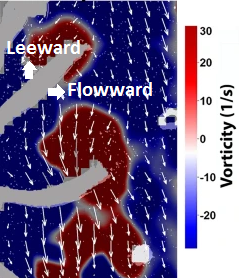
\includegraphics[width=.95\linewidth]{Figures/Vorticity.png}}
  \caption{Vorticity}
  \label{Vorticity}
\end{minipage}%
\begin{minipage}{0.33\textwidth}
  \centering\vspace{1.3mm}
  \frame{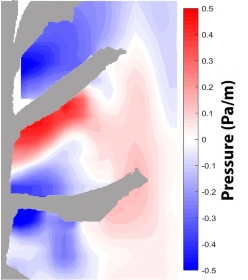
\includegraphics[width=.95\linewidth]{Figures/Pressure.png}}
  \caption{Pressure}
  \label{Pressure}
\end{minipage}
\begin{minipage}{0.33\textwidth}
  %\captionof{\textbf{c}}
  \centering\vspace{3mm}
  \frame{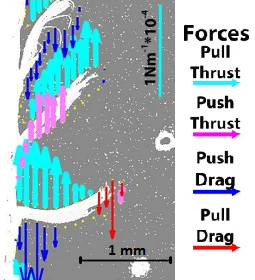
\includegraphics[width=.95\linewidth]{Figures/Forces.png}}
  \caption{Forces}
  \label{Forces}
\end{minipage}
\end{figure}
\begin{thebibliography}{1}
\bibitem{} 
Colin, S.P., Costello, J.H., Sutherland, K.R. "The role of suction thrust in the metachronal paddles of swimming invertebrates. Sci Rep 10, 17790 (2020)."
\\ \url{https://doi.org/10.1038/s41598-020-74745-y}
\end{thebibliography}
%\par The propulsors of these metachronal swimmers rely on generating negative pressure along their surfaces to generate forward thrust (i.e., \textbf{suction thrust}). Relying on negative pressure, as opposed to high pushing pressure, facilitates metachronal waves and enables these swimmers to exploit readily produced hydrodynamic structures. Surveys have shown that most animal propellers bend similarly in location() 



 

%An abundance of swimming animals have converged upon a common swimming strategy using multiple propulsors coordinated as metachronal waves. The shared kinematics suggest that even morphologically and systematically diverse animals use similar fluid dynamic relationships to generate swimming thrust. We quantified the kinematics and hydrodynamics of a diverse group of small swimming animals who use multiple propulsors, e.g. limbs or ctenes, which move with antiplectic metachronal waves to generate thrust. Here we show that even at these relatively small scales the bending movements of limbs and ctenes conform to the patterns observed for much larger swimming animals. We show that, like other swimming animals, the propulsors of these metachronal swimmers rely on generating negative pressure along their surfaces to generate forward thrust (i.e., suction thrust). Relying on negative pressure, as opposed to high pushing pressure, facilitates metachronal waves and enables these swimmers to exploit readily produced hydrodynamic structures. Understanding the role of negative pressure fields in metachronal swimmers may provide clues about the hydrodynamic traits shared by swimming and flying animals.

%A ciliary beat cycle consists of an effective stroke in which the extended cilium makes an oar-like movement towards one side, and a recovery stroke in which the cilium moves back by propagating a bend from base to tip.
%Broad surveys of propulsors of swimming and flying animals (e.g.; fins, wings, limbs) have shown that most animal propulsors bend similarly in location (inflexion point occurs ~ 0.65 along propulsor) and excursion (they bend ~ 27°)1. To understand the basis of these patterns we must better understand how propulsors interact with their surrounding fluid.
%propulsor maximizes the drag it generates during the power stroke and minimizes its drag during the recovery.
%The hydrodynamics around a moving propulsor generate a pressure field along the propulsor surface. The pressure gradient across the propulsor is the ultimate source of thrust necessary for swimming (and flying). Conventionally, it has been thought that these pressure fields are dominated by positive pressure generated as a propulsor pushes on the water and pushes the swimmer forward3. However, recent studies have shown that for some animals, including fish and jellyfish, it is actually negative pressure fields aligned along the leeward side of moving propulsors that dominates the pressure field and serve to essentially pull animals through the water (termed suction thrust4).  rows of fused cilia called ctenes
%This kinematic coordination of multiple propulsors has been proposed to be widespread because antiplectic metachronal waves enable each propulsor to move unobstructed by adjacent propulsors
% All of these animals swim using drag-based paddles with antiplectic metachronal kinematics and at Reynolds numbers (based on appendage length) ranging from 17 to 95
 %he ctenes and limbs of the five species analyzed bent similarly during their power stroke, whereby, (a) the mean bending angle among all the species was 27° ± 6.1 (mean shown by solid line and s.t. dev. shown by dashed line) and (b) the mean inflexion point among all the species was located 0.59 ± 0.045 along the the limb/ctene. 
%  peak water flow (i.e., maximum flow velocity) was located near the inflexion point occurring on average at 0.68 ± 0.1 along the limb/ctene. In addition, (e) water flow was on average 1.31 ± 0.22 times greater on the leeward side of the limb/ctene than the flowward side (blue dashed line shows unity). The (f) average negative pressure along the length of the leeward side of the limb/ctene was 5.65 ± 3.3 times greater than the average positive pressure along the flowward side
%  peaked in the proximity of the bending inflexion point rather than at the very tip of the propulsor (Fig. 2d; peak flow location = 68.4% ± 10.0).
%   velocities on the leeward side of the propulsors were greater than on the flowward side
 %  These velocity fields are different than velocities around rigid paddles where peak velocities occur at the very tip and on  the flowward side of the propulsors
 %  Pressure fields around the bending propulsors (Fig. 3d–f) revealed that these %velocity characteristics were related to strong negative pressure regions along the leeward side of the propulsors (Figs. 2f, 3d–f). Weaker positive pressure regions were observed on the flowward sides of the propulsors. Throughout the propulsors’ power stroke, negative pressure was much greater than positive pressure (Fig. 2f), which meant the limbs and ctenes pulled a bulk of fluid toward the rearward direction relative to the animal’s trajectory.
 %  Representative PIV, pressure and force vectors of (a,d,g) the ctenophore Pleurobrachia bachei, (b,e,h) the polychaete annelid Tomopteris sp. and (c,f,i) an unidentified larval decapod arthropod swimming up. The deep blue areas in the pressure frames (d–f) indicate areas of strong negative pressure. The aquamarine force vectors show the predominance of the pulling forces acting on the limbs/ctenes during the power stroke. Scale bars along the bottoms show 1 mm length
%   Pressure values along the surface of the propulsors can be used to estimate the thrust and drag acting on the propulsors throughout their power strokes (Fig. 3g–i). The negative pressures on the leeward side of the propulsors resulted in all the propulsors predominately pulling the animals forward rather than pushing the animals forward (Fig. 4a–d). Time series of the forces during the power stroke showed that the pushing forces initially, and briefly, peaked as the propulsors began their stroke, but, for the majority of the power stroke the propulsors were primarily pulling the animals forward (Fig. 4a–c). As a result, the sum of the forces acting on the propulsor throughout the power stroke showed that the pulling forces strongly dominated the forces generated by the metachronal propulsors. Among all the ctenophores, arthropods and the annelid examined, the pulling forces were 2 to 34 times greater than the pushing forces generated by the metachronal propulsors 
 %  Bending at propulsor margins encourages vortex formation on the lee side of the propulsor (Figs. 2, 3) that differs from rigid propulsors. Counter-rotating vortices formed on the lee side of a bending propulsor accelerate fluid at the intersection of the vortices12,15. The fluid thus accelerated relative to the leading edge of the propulsor is the basis of the pressure gradient across the propulsor surface. In turn, this elevated pressure gradient generates high thrust and is the reason for the dominant contribution of suction thrust to natural bending propulsors
%   Bending kinematics in particular have been shown to greatly enhance vorticity and along with that, negative pressure11,16,17. Rigid, non-bending paddles generate different hydrodynamic structures than we observed13,14 and do not generate strong negative pressure fields16,17,18,19. Therefore, the kinematics of bending appear to be important for generating strong negative pressure fields around moving propulsors.
%   In addition to the benefits for single propulsors, negative pressure fields can facilitate the movement and coordination of multiple propulsors which have antiplectic metachronal wave kinematics. During an antiplectic metachronal wave, a leading propulsor will begin the power stroke and, after it has initiated its stroke, the propulsor immediately behind it will initiate its own power stroke. This sequential pattern will continue for all the subsequent propulsors in the antiplectic wave. The predominately negative pressure on the leeward of each propulsor can serve to facilitate the kinematics of the adjacent propulsor by reducing the hydrodynamic resistance necessary to initiate and complete its power stroke26. In addition, the negative pressure in the gap between adjacent propulsors can serve as a cue for the adjacent propulsor to initiate its power stroke. 
%   The limbs and ctenes of small invertebrates rely on the generation of negative pressure fields for thrust production and their bending kinematics conform to the bending patterns observed among a vast array of swimming and flying animals. This may reflect the fact that a subtle bend (< 30% inflexion) appears to generate a cascade of hydrodynamic effects which enhance formation of negative pressure regions around propulsors and, ultimately, lead to enhanced thrust and hydrodynamic efficiency. These enhancements appear to be optimized for small bends20,21. Invertebrate animals with multiple paddles can coordinate the sequential build-up of negative pressure fields along antiplectic metachronally moving limbs for an additive thrust benefit and to facilitate the coordination of the sequential propulsors.

 
%\end{multicols}

\end{document}